\documentclass{../../slides-style}

\usepackage{colortbl}

\slidetitle[Лекция 1: О программной инженерии]{Технология разработки программного обеспечения}{11.02.2025}

\begin{document}

    \begin{frame}[plain]
        \titlepage
    \end{frame}

    \section{Организационное}

    \begin{frame}
        \frametitle{Организационное}
        \begin{itemize}
            \item Лекционный курс, с одной \enquote{контрольной}
            \begin{itemize}
                \item На самом деле, практика на паре с небольшим баллом
            \end{itemize}
            \item В конце зачёт
            \begin{itemize}
                \item Примерно 70 вопросов без подготовки
            \end{itemize}
            \item Балльная система ECTS
            \begin{itemize}
                \item 80 баллов за зачёт, 20 баллов за практическую работу
            \end{itemize}
            \item Материалы будут выкладываться в HwProj, туда же сдавать практическую работу
            \begin{itemize}
                \item \url{https://hwproj.ru/courses/40027}
            \end{itemize}
            \item Коммуникация в Teams, в отдельном канале в команде курса
        \end{itemize}
    \end{frame}

    \begin{frame}
        \frametitle{Что будет в курсе}
        \begin{itemize}
            \item Что в разработке программного обеспечения делается помимо программирования, кем ещё можно работать после матмеха
            \item Работа с требованиями
            \item Жизненный цикл программного обеспечения
            \item Методологии разработки, Scrum
            \item Проектирование пользовательских интерфейсов
            \item Управление проектами: что делают менеджеры
            \item Работа в команде
            \item Качество программного обеспечения, работа с дефектами
            \item Сопровождение и поддержка, развитие проектов после релиза
            \item Рефакторинг (если успеем)
            \item Непрерывная интеграция/непрерывное развёртывание
            \item Экономические аспекты разработки
        \end{itemize}
    \end{frame}

    \section{Введение}

    \begin{frame}
        \frametitle{Программа и программный продукт}
        \begin{center}
            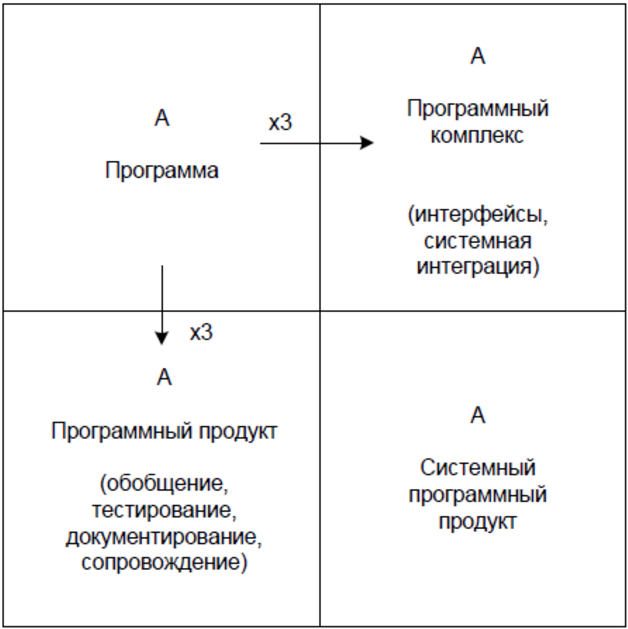
\includegraphics[width=0.5\textwidth]{brooksSquare.png}
        \end{center}
        \begin{textblock}{2}(9.5,-4)
            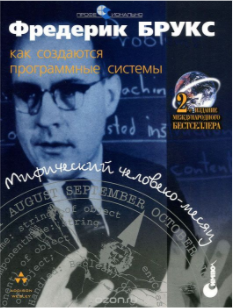
\includegraphics[width=\textwidth]{brooksCover.png}
        \end{textblock}
    \end{frame}

    \begin{frame}
        \frametitle{Особенности промышленной разработки ПО}
        \begin{itemize}
            \item Работа в команде
            \item Работа для заказчика и за деньги
            \item Требования, сроки и качество
            \item Поэтому нужны дополнительные действия:
            \begin{itemize}
                \item Анализ и проектирование
                \item Выбор технологий и планирование
                \item Организация процесса разработки
                \item Учёт необходимости сопровождения и интеграции, документирование, стайлгайд
                \item Формирование команды, подбор персонала, оборудования и помещений
                \item ...
            \end{itemize}
        \end{itemize}
    \end{frame}

    \begin{frame}
        \frametitle{Программная инженерия как область знания}
        \begin{itemize}
            \item Организация и улучшение процесса разработки ПО, управление коллективом разработчиков, разработка и внедрение средств поддержки жизненного цикла разработки ПО
            \item Осмысление, обобщение и оформление опыта
            \item Методы и практики тестирования, проектирования, работы над требованиями и т.п.
            \item Стандарты и методологии
        \end{itemize}
    \end{frame}

    \section{Немного истории}

    \begin{frame}
        \frametitle{Истоки: ENIAC}
        \begin{columns}
            \begin{column}{0.5\textwidth}
                \begin{itemize}
                    \item ENIAC~--- Electronic Numerical Integrator and Computer 
                    \item Программирование происходило физически тумблерами и штекерами
                    \item Порог вхождения очень высок
                    \item Программ отдельно от компьютеров не существовало
                    \item Управлять процессом не требовалось вообще
                \end{itemize}
            \end{column}
            \begin{column}{0.5\textwidth}
                \begin{center}
                    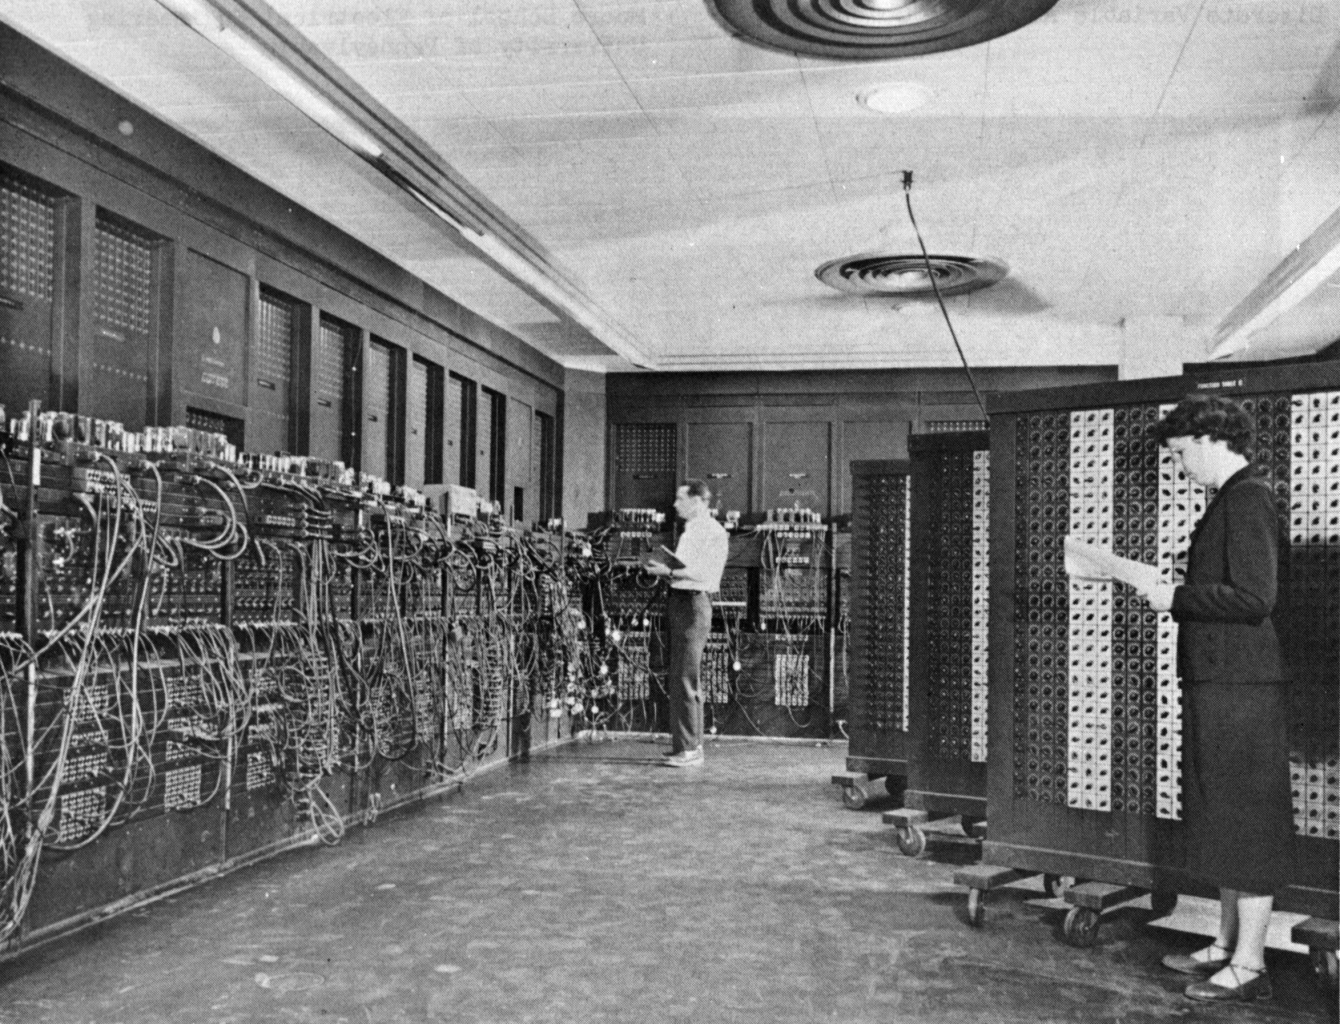
\includegraphics[width=\textwidth]{eniac.png}
                \end{center}
            \end{column}
        \end{columns}
    \end{frame}

    \begin{frame}
        \frametitle{Взрывной рост разработки}
        \framesubtitle{Появление языков высокого уровня}
        \begin{columns}
            \begin{column}{0.5\textwidth}
                \begin{itemize}
                    \item 1957~--- Fortran (Formula Translator)
                    \item Начало массовой разработки на заказ
                    \item Процесс управления разработкой ``Code \& Fix'' (также известный как Cowboy Coding)
                    \item ПО всё ещё привязано к ``железу''
                    \item Стандартов разработки нет
                \end{itemize}
            \end{column}
            \begin{column}{0.5\textwidth}
                \begin{center}
                    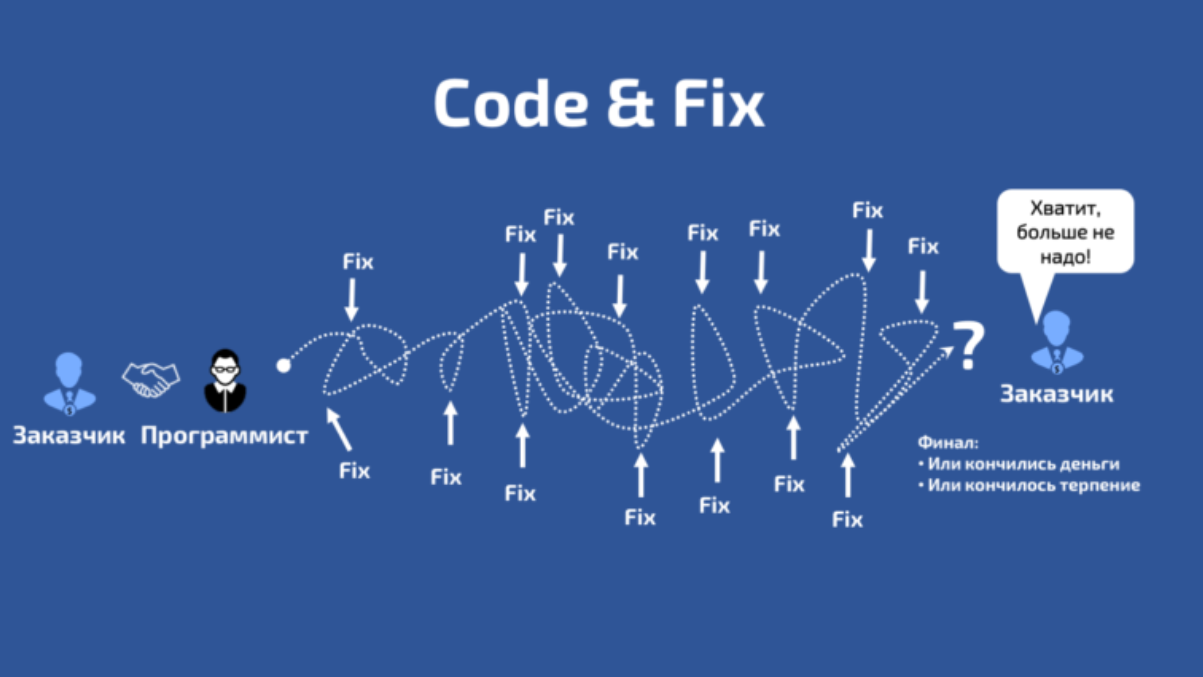
\includegraphics[width=\textwidth]{codeAndFix.png}
                \end{center}
            \end{column}
        \end{columns}
    \end{frame}

    \begin{frame}
        \frametitle{Первая попытка навести порядок}
        \framesubtitle{Официальное рождение программной инженерии}
        \begin{columns}
            \begin{column}{0.7\textwidth}
                \begin{itemize}
                    \item Кризис программного обеспечения
                    \begin{itemize}
                        \item Стоимость проектов превышает бюджет
                        \item Превышаются сроки выполнения проектов
                        \item ПО слишком неэффективно
                        \item ПО имеет слишком низкое качество
                        \item ПО не отвечает необходимым требованиям
                        \item Неуправляемые проекты, трудности с поддержкой кода
                        \item ...
                    \end{itemize}
                    \item конференция NATO Software Engineering
                    \begin{itemize}
                        \item Оборонка страдала больше всех
                    \end{itemize}
                \end{itemize}
            \end{column}
            \begin{column}{0.3\textwidth}
                \begin{center}
                    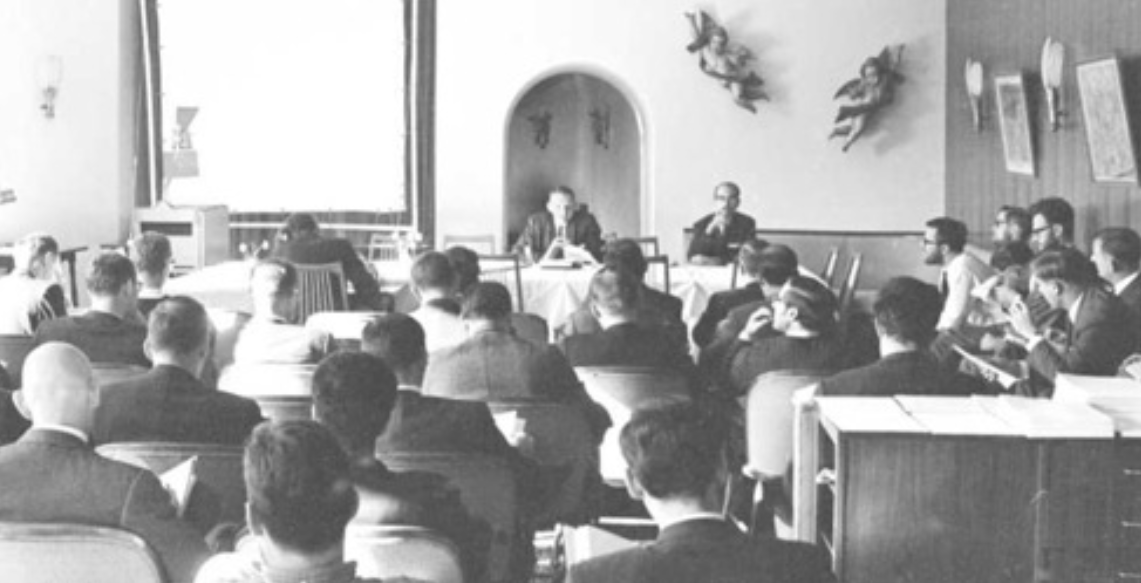
\includegraphics[width=\textwidth]{natoConference.png}
                \end{center}
            \end{column}
        \end{columns}
    \end{frame}

    \section{Немного статистики}

    \begin{frame}
        \frametitle{Текущее положение дел}
        \framesubtitle{Standish Group 2015 Chaos Report}
        \begin{center}
            \begin{tabu} {| X[2 l p] | X[1 c p] | X[1 c p] | X[1 c p] | X[1 c p] | X[1 c p] |}
                \tabucline-
                \everyrow{\tabucline-}
                                    & 2011 & 2012 & 2013 & 2014 & 2015 \\
                Successful          & 29\% & 27\% & 31\% & 28\% & 29\% \\
                Challenged          & 49\% & 56\% & 50\% & 55\% & 52\% \\
                Failed              & 22\% & 17\% & 19\% & 17\% & 19\% \\
            \end{tabu}
        \end{center}
    \end{frame}

    \begin{frame}
        \frametitle{Chaos resolution by project size}
        \begin{center}
            \begin{tabu} {| X[2 l p] | X[1 c p] | X[1 c p] | X[1 c p] |}
                \tabucline-
                \everyrow{\tabucline-}
                          & Successful & Challenged & Failed \\
                Grand     & 2\%        & 7\%        & 17\%   \\
                Large     & 6\%        & 17\%       & 24\%   \\
                Medium    & 9\%        & 26\%       & 31\%   \\
                Moderate  & 21\%       & 32\%       & 17\%   \\
                Small     & 62\%       & 16\%       & 11\%   \\
                Total     & 100\%      & 100\%      & 100\%  \\
            \end{tabu}
        \end{center}
    \end{frame}

    \section{Отличия от других областей}

    \begin{frame}
        \frametitle{Отличия от других областей производства}
        \begin{itemize}
            \item Очень высокая сложность систем
            \begin{itemize}
                \item \url{http://www.informationisbeautiful.net/visualizations/million-lines-of-code/}
            \end{itemize}
            \item Меньше накоплено опыта
            \begin{itemize}
                \item Более непредсказуем результат
                \item Хуже поддается планированию
                \item Больше творчество, чем ремесло
            \end{itemize}
            \item Подверженность постоянным изменениям
            \item Но и стоимость изменений значительно ниже
        \end{itemize}
    \end{frame}

    \begin{frame}
        \frametitle{Разработка ПО крайне социализирована}
        \begin{itemize}
            \item Разработка ведётся людьми
            \begin{itemize}
                \item Общение внутри команды
            \end{itemize}
            \item Разработка ведётся для людей
            \begin{itemize}
                \item Общение за пределами команды
            \end{itemize}
            \item Успех определяется социальными факторами
            \begin{itemize}
                \item Технологии вторичны?
            \end{itemize}
        \end{itemize}
    \end{frame}

    \begin{frame}
        \frametitle{Команда}
        \begin{center}
            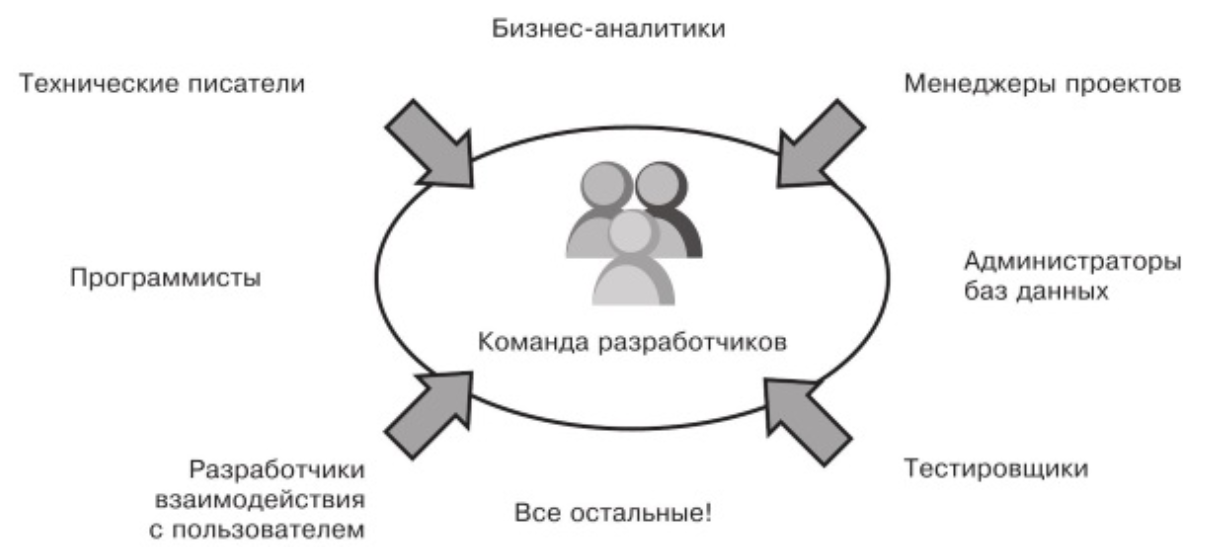
\includegraphics[width=0.8\textwidth]{team.png}
        \end{center}
    \end{frame}

    \section{Профстандарты}

    \begin{frame}
        \frametitle{Востребованные компетенции}
        \begin{itemize}
            \item Умение работать в команде
            \item Владение современными стратегиями и технологиями организации коллективной разработки программного обеспечения, включая системы управления версиями, процессы непрерывной интеграции, стандарты оформления кода и методы инспекции кода
            \item Понимание основных направлений развития методов коллективной разработки, их отличий и целесообразности применения в зависимости от типа решаемых задач и требований организации
            \item Владение более чем одним языком программирования/стеком технологий
        \end{itemize}
    \end{frame}

    \begin{frame}
        \frametitle{Профстандарты}
        \begin{itemize}
            \item Собрание трудовых функций, знаний и умений для данной профессии, относительно которых есть консенсус в индустрии
            \item Разрабатываются комитетами из крупных компаний, утверждаются Минтруда
            \item Нужны прежде всего для стандартизации требований и подготовки
            \begin{itemize}
                \item В перспективе~--- стандартизованной сертификации
            \end{itemize}
            \item Разбиты на уровни квалификации
            \begin{itemize}
                \item Всего 9 уровней, от неквалифицированного труда до ``управления крупными техносистемами, генерации фундаментальных знаний''
                \item Диплом бакалавра~--- с шестого, магистерский~--- с седьмого
                \item Девятый уровень требует окончания аспирантуры
            \end{itemize}
        \end{itemize}
    \end{frame}

    \begin{frame}
        \frametitle{Профстандарт <<Программист>>, 3-й уровень квалификации}
        \framesubtitle{Минимальный. Низкоквалифицированный труд}
        \begin{itemize}
            \item Формализация и алгоритмизация поставленных задач для разработки программного кода
            \item Написание программного кода с использованием языков программирования, определения и манипулирования данными в базах данных
            \item Оформление программного кода в соответствии с установленными требованиями
            \item Работа с системой управления версиями программного кода
            \item Проверка и отладка программного кода
        \end{itemize}
    \end{frame}

    \begin{frame}
        \frametitle{Профстандарт <<Программист>>, 4-й уровень квалификации}
        \framesubtitle{<<Миддл>>}
        \begin{itemize}
            \item Разработка процедур проверки работоспособности и измерения характеристик компьютерного программного обеспечения
            \item Разработка тестовых наборов данных для проверки работоспособности компьютерного программного обеспечения
            \item Проверка работоспособности компьютерного программного обеспечения
            \begin{itemize}
                \item \emph{Да-да, тестировщик должен иметь большую квалификацию, чем программист}
            \end{itemize}
            \item Рефакторинг, оптимизация и инспекция программного кода
            \item Исправление дефектов программного кода, зафиксированных в базе данных дефектов
            \item Осуществление сборки однородных программных модулей в программный проект
        \end{itemize}
    \end{frame}

    \begin{frame}
        \frametitle{Профстандарт <<Программист>>, 5-й уровень квалификации}
        \begin{itemize}
            \item Разработка процедур интеграции программных модулей
            \item Осуществление интеграции программных модулей и компонентов и проверки работоспособности выпусков программного продукта
        \end{itemize}
    \end{frame}

    \begin{frame}
        \frametitle{Профстандарт <<Программист>>, 6-й уровень квалификации}
        \framesubtitle{<<Сеньор>>}
        \begin{itemize}
            \item Анализ возможностей реализации требований к компьютерному программному обеспечению
            \item Разработка технических спецификаций на программные компоненты и их взаимодействие
            \item Проектирование компьютерного программного обеспечения
        \end{itemize}
    \end{frame}

    \begin{frame}
        \frametitle{Какие ещё профстандарты учитываются}
        \begin{footnotesize}
            \begin{itemize}
                \item 06.003 <<Архитектор программного обеспечения>>
                \item 06.004 <<Специалист по тестированию в области информационных технологий>>
                \item 06.011 <<Администратор баз данных>>
                \item 06.015 <<Специалист по информационным системам>>
                \item 06.019 <<Технический писатель (специалист по технической документации в области информационных технологий)>>
                \item 06.022 <<Системный аналитик>>
                \item 06.026 <<Системный администратор информационно-коммуникационных систем>>
                \item 06.028 <<Системный программист>>
                \item 40.011 <<Специалист по научно-исследовательским и опытно-конструкторским разработкам>>
                \item 40.057 <<Специалист по автоматизированным системам управления производством>>
            \end{itemize}
        \end{footnotesize}
    \end{frame}

    \section{SWEBOK}

    \begin{frame}
        \frametitle{Software Engineering Book of Knowledge}
        \begin{footnotesize}
            \begin{enumerate}
                \item Software Requirements
                \item Software Design
                \item Software Construction
                \item Software Testing
                \item Software Maintenance
                \item Software Configuration Management
                \item Software Engineering Management
                \item Software Engineering Process
                \item Software Engineering Models and Methods
                \item Software Quality
                \item Software Engineering Professional Practice
                \item Software Engineering Economics
                \item Computing Foundations
                \item Mathematical Foundations
                \item Engineering Foundations
            \end{enumerate}
        \end{footnotesize}
    \end{frame}

\end{document}
